\chapter{SPRR: Steady State Filtration }


\subsection{Experimental Design}
\rod{et bud på at rykke overvejelser og korte det ned.}
A multi factor experiment was designed to investigate the rejection of \ce{Cl-} and \ce{SiO2} with changing environment.
The same lab-scale filtration set-up and filtration parameters as described in \textcolor{blue}{ref til et afsnit} was used, but with a single pass filtration configuration.
Steady state is an important premise for the single pass experimental setup, therefore each filtration was run for as long time needed for steady state to occur. 
%In order to achieve steady state the experiments were run in different experimental configuration, as described in \textcolor{blue}{singlepass afsnittet eller flyt det her ned}. 
%50 L synthetic CT water was made and if needed both concentrate and permeate was recycled to the feed tank
50 L synthetic CT water was produced where a configuration with recycling of concentrate and permeate, or no recycling could occur depending on filtration time needed to reach steady state. 
A factorial design approach was used where all possible combination of various factors at different levels are investigated, this allows investigation of both main effects of each factor, but also of possible interaction effects.  \citep{DesignOfExperiments_book_bruno}
The factorial experiment gives more information at fewer experiments and therefore is generally more efficient than other experimental designs e.g. best guess approach, especially as the number of factors increases. \citep{DesignOfExperiments_book_bruno} 
%This also means that with increasing number of factors and levels the number of experiments required quickly rises to unpractical levels. 
This experiment focused on factors which are theorized to impact the rejection of chloride and silica. 

%As previously mentioned in \textcolor{blue}{tænker der kommer noget i teori} the anion combination greatly influences the rejection of the monovalent chloride ions. 
Different ratios of chloride to sulphate was investigated . 
Silica most likely also influences the anion rejection specifically at high pH where silica can achieve a negative charge and can possibly impact the charge balance, \textcolor{blue}{as mentioned in theory omkring silica}.
The factors which are theorized to have the largest impact and possible interaction effects are therefore: change in chloride to sulphate ratio, silica concentration and pH, which will be combined at different levels for each experiment according to \cref{tab:SPRR_factors_levels}. 
The chloride and sulphate ratio was investigated at at three different levels 25 \%, 50 \% and 75\% chloride, with a chloride concentration at 5 mM for all experiments, and adjusted sulphate level accordingly to reach the desired ratio. 
The silica concentration will be investigated at high and low content.
%Furthermore when determining the different levels of each factor it was discovered that the factors influence each other, where higher silica concentration gives rise to increase in pH, and as pH was adjusted with hydrochloric acid  and sodium hydroxide this would influence the chloride and sulphate ratio. 
As with the \textcolor{blue}{ref til multisalt forsøg} the pH will be adjusted by use of a carbonate-bicarboante buffer system, where a 0.008 M buffer with pH of 9.25 will be used for all experiment, and hydrochloric acid will be used to adjust to desired pH.
This is done to keep the sodium content as equal as possible between experiments. 
It was impossible to keep the sodium and calcium ratio identical between the experiments, while also varying the chloride-sulphate ratio, pH and silica level as these factors influence each other. 
Therefore, the sodium and calcium ratio will be kept high at >95\%.
Apart from these factors other parameters of the experiment will be kept constant.

%The cation ratio between calcium and sodium might also affect the rejection of chloride, but most CT operate with softened water, where the sodium to calcium ratio is high \textcolor{blue}{95\% hvad er den rigtigt}. 
%Therefore it was \textcolor{blue}{theorized/kilde} that this ratio might have a lower impact on the chloride and silica rejection, and will not be investigated in this experiment. 

\begin{table}[H]
\centering
\caption{Factors and levels for the multi factor single pass experiment}
\label{tab:SPRR_factors_levels}
\rowcolors{2}{gray!25}{white}
\begin{tabular}{l|ccc}
\rowcolor{gray!50}
  &  & \textbf{Factors} &   \\ 
  \rowcolor{gray!50}
\textbf{Level}   & \textbf{Cl \%} & \textbf{pH} & \textbf{Silica mg/L}  \\ \hline
1   & 25             & 9.25  & 125    \\
2   & 50               & 9.5   & -      \\
3  & 75               & 9.75  & 75    \\
\end{tabular}
\end{table}
 
 
\subsection{Data Processing} 

When analyzing the feed solution of the various filtrations, as measured by IC, the ion concentrations deviated from the assumed theoretical feed concentration. 
Only the sulphate and silica concentrations were close to their assumed theoretical values. 
Calcium was the species with the largest deviation assumed to be 0.5 mM for all filtration but instead varied from 0.04-0.2 mM, being significantly lower.
This gave a larger \ce{Na/(Ca+Na)} ratio than expected of >98\%, despite all measured sodium concentrations being lower than the theoretical concentrations.
The measured chloride concentrations did not deviate much from the assumed value of 5 mM with exception for one filtration which had a concentration 2.1 mM, changing the \ce{Cl/(SO4+Cl)} value significantly.
Therefore solely the measured values will be used in further data processing. 
This deviation could be caused by imprecise measurement of water volume used to dissolve the species, or due to uncertainty of the IC analysis. 

\textbf{Silica rejection }\\
As also explored in \textcolor{blue}{Complex ion matrix} the rejection of silica is influenced by pH changes. 
This was explored further during this experiment where the anion ratio also was varied as well as pH. 
From \cref{fig:Silica_rejection_3D} it is evident that both higher pH and \ce{Cl^-/(Cl^- + SO4^{2-})} ratio leads to higher silica rejection which varies from 15-44 \%. The change in pH from 9.26 to 9.89 has a much larger effect on silica rejection compared to change in \ce{Cl^-/(Cl^- + SO4^{2-})} ratio. 
The concentration of silica was investigated at high and low level where a higher concentration of Silica in the feed stream also leads to higher silica rejection. 

\begin{figure}[H]
    \centering
    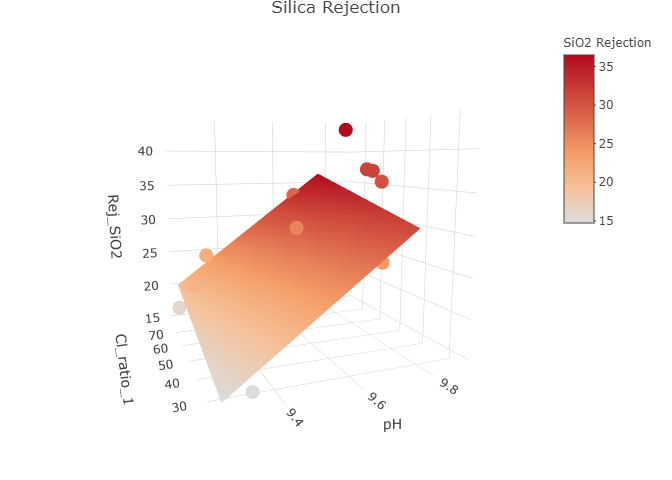
\includegraphics[width=0.8\textwidth]{Billeder/data/SPRR/Silica_rejection_3D.png}
    \caption{Silica rejection against pH and \ce{Cl^-/(Cl^- + SO4^{2-})}}
    \label{fig:Silica_rejection_3D}
\end{figure}


\textbf{Chloride rejection }\\

The measured rejection of chloride varied from -23\% to 18\%, and seems to be influenced by the anion ratio, where the \ce{Cl^-/(Cl^- + SO4^{2-})} ratio was varied from 25\% to 75\%, see \cref{fig:Chloride_rejection_3D}. 
With a higher \ce{Cl^-/(Cl^- + SO4^{2-})} ratio a higher rejection of chloride is achieved, only two filtrations had higher \ce{SO4^2-} content than \ce{Cl-} and these filtrations showed negative \ce{Cl-} rejection. 
pH also seems to have an influence on the rejection of chloride, where a higher pH leads to slightly higher chloride rejection, which is in contrast to what was theorized when considering the higher fraction of charged \ce{SiO2} at a higher pH. 
The level of \ce{SiO2} present did not seem to influence the chloride rejection.
pH had a much lower impact on chloride rejection compared to the anion ratio. 


\begin{figure}[H]
    \centering
    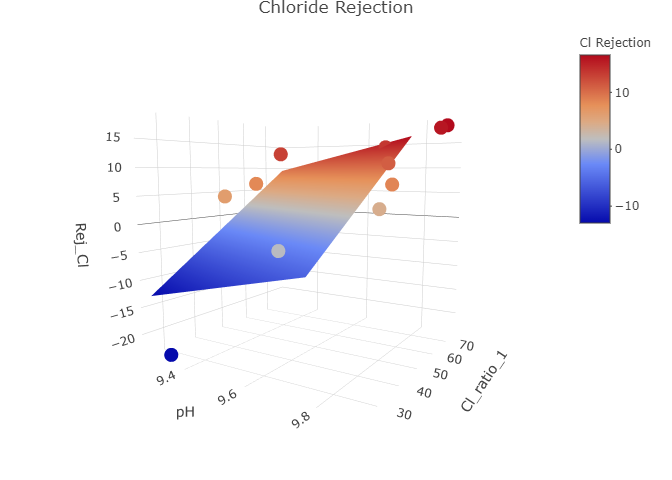
\includegraphics[width=0.8\textwidth]{Billeder/data/SPRR/Chlorid_rejection_3D.png}
    \caption{Chloride rejection against pH and \ce{Cl^-/(Cl^- + SO4^{2-})}}
    \label{fig:Chloride_rejection_3D}
\end{figure}

\textcolor{blue}{noget mere om anion rejection here eller vent med det til model?}


\textbf{Calcium}
The calcium rejection was affected by chloride content at higher concentrations of silica.
Calcium rejection varied from 37\% - 94\%, but due to the low concentrations detected in the feed stream the calcium analysis has higher uncertainty than the other  measured species. 
\textcolor{blue}{hvorfor svinger den så meget, og umildbart er det ikke grundet Cl, SiO2 eller pH... men da Ca også varierede meget i feed conc er det måske upålideligt.Jeg har indsat det billede der giver mest mening, men der mangler en tendens.}

\begin{figure}[H]
    \centering
    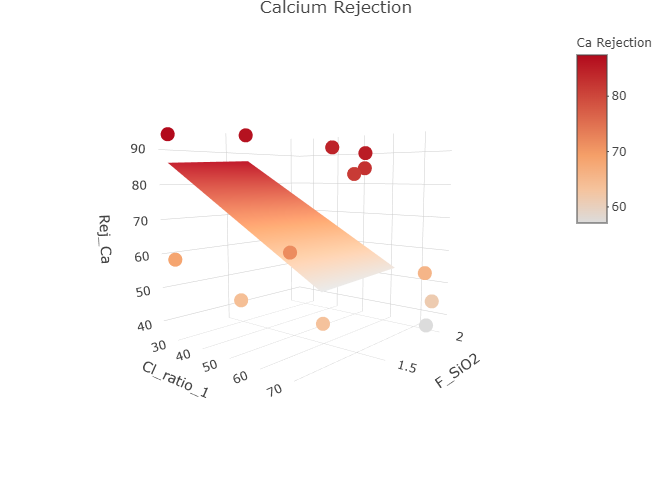
\includegraphics[width=0.8\textwidth]{Billeder/data/SPRR/Calcium_rejection_3D.png}
    \caption{Calcium rejection against pH and \ce{Cl^-/(Cl^- + SO4^{2-})}}
    \label{fig:Calcium_rejection_3D}
\end{figure}

\textbf{Sodium}\\
Sodium rejection varied from 47\% - 73\%, and is influenced by the anion ratio where a lower \ce{Cl^-/(Cl^- + SO4^{2-})} content leads to higher sodium rejection. 
Increase in pH leads to increase in sodium rejection. 
\textcolor{blue}{Det tror jeg ikke jeg forstår hvorfor. }

\begin{figure}[H]
    \centering
    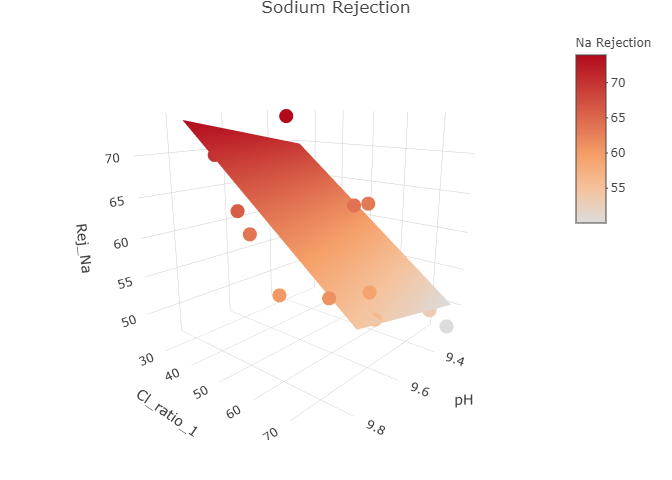
\includegraphics[width=0.8\textwidth]{Billeder/data/SPRR/Sodium_rejection_3D.png}
    \caption{Chloride rejection against pH and \ce{Cl^-/(Cl^- + SO4^{2-})}}
    \label{fig:Sodium_rejection_3D}
\end{figure}



\textbf{Sulphate}\\
Like previous experiment sulphate had the highest rejection which varied from 94\% - 99\%. 
This small decrease in sulphate rejection seemed to be due to increase in chloride content. 



\textbf{Bicarbonat}
forsøg nr. 11 (pH 9,5, silica 125 mg/L og 50 Cl \%) har lavere feed end permeat, derfor negativ rejection, jeg kan ikke lige lure hvad der er gået galt der..... 
Vi troede 17 prøven var feed i stedet for permeat (som der stod på den) men den har værdi på 130 mg/L så det er nok rigtig nok med permeat.
\rod{Bicarbonat sejler, jeg har ikke kigget på det.}










\textbf{Gammelt data behandling. }


%%%%Lærke Statisik:
tukey når der kun er en replicate. se side 242 for eksempler på ligniner for effect. 

data behandling: for Cl rejection. 
hvis forsøget betrages som $2^3$ og kun 2 levels af pH undersøges mod hinanden får man. 

pH 9.25, 9.5
main effect, Cl, SiO2 og pH
interaktion effect ml. Cl og SiO2. 

pH 9.5, 9.75
main effect, Cl og pH
interaktion effect ml. silica og Cl, samt interaktion ml. SiO og pH. 

pH 9.25, 9.75
main effect, Cl,  pH
interaktion effect ml. silica og pH. 

Se excel ark: statistik SPRR.
%%%%
% \prettyinpink{Generelt er alle Na ratio >99\% men det er ikke sååå stort et problem.\\
% De fleste Cl værider/ratioer passer på det de burde være med undtagelse af: nr 8 der kun er 25\% (burde være 50 og 15 der er 66\% og burde være 75\%}

\textbf{Afsnit}\\

\begin{figure}[H]
    \centering
    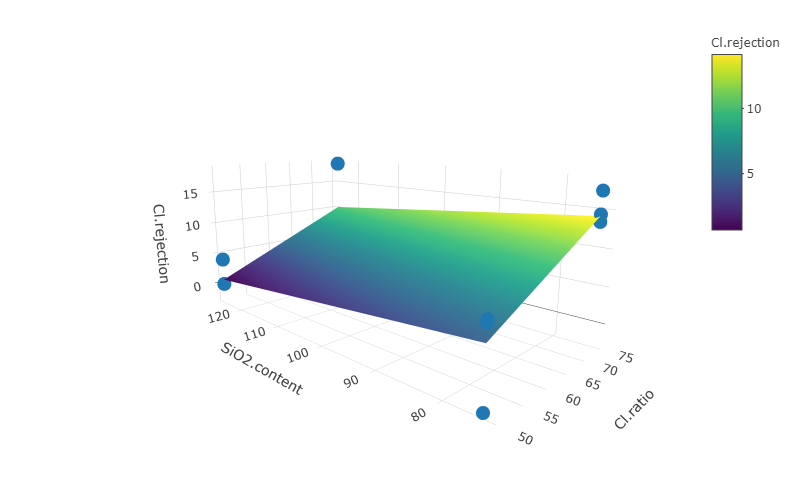
\includegraphics[width=0.8\textwidth]{Billeder/data/SPRR/cl_ratio_sio2_conc_cl_rejection_3d.png}
    \caption{I made this :) It's bad :(}
    \label{fig:3d plot}
\end{figure}
For the following data is presented as ion rejections as a function of chloride content as a ratio between chloride and sulfate as this is assumed to be important for the rejections at least for chloride.
It is also possible that chloride content as a ratio between chloride and all other anions would give better understanding.
The required information is difficult to obtain as bicarbonate concentrations are hard to accurately acquire plus the fact that the degree to which silica is charged is obscured.
Assuming that chloride is more affected by divalent anions only including sulfate may be a good enough approach....  


